%%%%%%%%%%%%%%%%%%%%%%%%%%%%%%%%%%%%%%%%%%%%%%%%%%%%%%%%%
%%%
%%%  第3章
%%%  図表等の挿入
%%%
%%%%%%%%%%%%%%%%%%%%%%%%%%%%%%%%%%%%%%%%%%%%%%%%%%%%%%%%%
Moonbot, designed for lunar surface operations, relies on a sophisticated software foundation. This chapter describe the structure of Moonbot's software architecture and the used tools.

%%%%% ROS2 %%%%%
\section{Software Tools}
\subsection{ROS and ROS2}
\textbf{ROS (Robot Operating System):} \cite{ros} is a flexible framework for writing robot software. ROS provides services for hardware abstraction, device drivers, communication between processes, package management, and more. ROS has been widely adopted in the robotics community, fostering collaboration and the sharing of libraries and tools.

\textbf{ROS2 (Robot Operating System 2):} The next generation of ROS, ROS2 \cite{ros2} is designed to address limitations and capitalize on the lessons learned from the widespread use of its predecessor. One of the significant improvements in ROS2 is its enhanced support for the Data Distribution Service (DDS) middleware \cite{DDS}. DDS is a standardized communication middleware that facilitates efficient and reliable data exchange between distributed systems. 

By the above information, Moonbot utilizes ROS2, Foxy distribution, as the primary tool for organizing communication among its modular components. The decision to use ROS2 is motivated by its enhanced features, including:

\begin{itemize}
\item \textbf{Real-Time Capabilities:} ROS2 provides improved support for real-time systems, crucial for dynamic and responsive control.
\item \textbf{Communication Middleware:} ROS2 offers a communication middleware options, allowing components to exchange information in a distributed system.
\item \textbf{Modularity and Extensibility:} The modular and extendable structure allow developer to debug or extend the feature of the program easily.
\end{itemize}
%%%

\subsection{ROS2 Core Concepts and Elements}
\subsubsection{ROS2 Graph}
In ROS. it provide a communication network called  ``ROS graph". ROS2 process all data and connect them simultaneously via ROS2 graph. Develop utilize this concept to map the ROS2 elements to execute the program.\\

\begin{figure}[h]
  \centering
  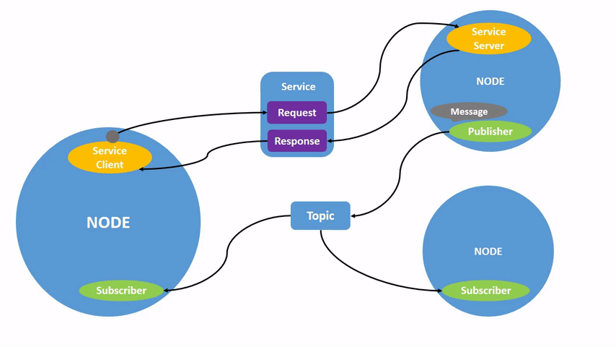
\includegraphics[width=120mm]{./fig/chap3/node.png}
  \vspace{2mm}
  \caption{Visualization of ROS2 graph. \cite{ros2}}\label{ros2_graph}
\end{figure}

\subsubsection{ROS2 Nodes}
Nodes are individual processes in a ROS 2 system. They communicate with each other by publishing and subscribing to topics, providing and using services, and executing actions.

\subsubsection{ROS2 Topics}
Topics are named buses over which nodes can exchange messages. A node can publish messages to a topic, and any other node can subscribe to that topic to receive those messages. Topics facilitate asynchronous communication between nodes.
 
\subsubsection{ROS2 Services}
Services allow request-response communication between nodes. A node provides a service by specifying a request message type and a response message type. Other nodes can then call that service by sending a request message and receiving a response message.
 
\subsubsection{ROS2 Actions}
Actions provide a way for nodes to execute long-running tasks in a goal-oriented manner. Actions consist of a goal, feedback, and result, allowing for more complex interaction patterns than services. Nodes can send action goals, receive feedback on the progress of those goals, and eventually receive a result once the goal is completed.\\
%%%%% ROS2 %%%%%

%%%%% ROS2 CONTROL %%%%%
\subsection{ROS2 Control}
Moonbot's control architecture is developed with ROS2, and within this framework, the ROS2 control package \cite{ros2control} plays a key role. In this section, we are going to delve into the specifics of ROS2 control, its integration with Moonbot's control system, and the key components that contribute to Moonbot's adaptability and precision.

\begin{figure}[ht]
  \centering
  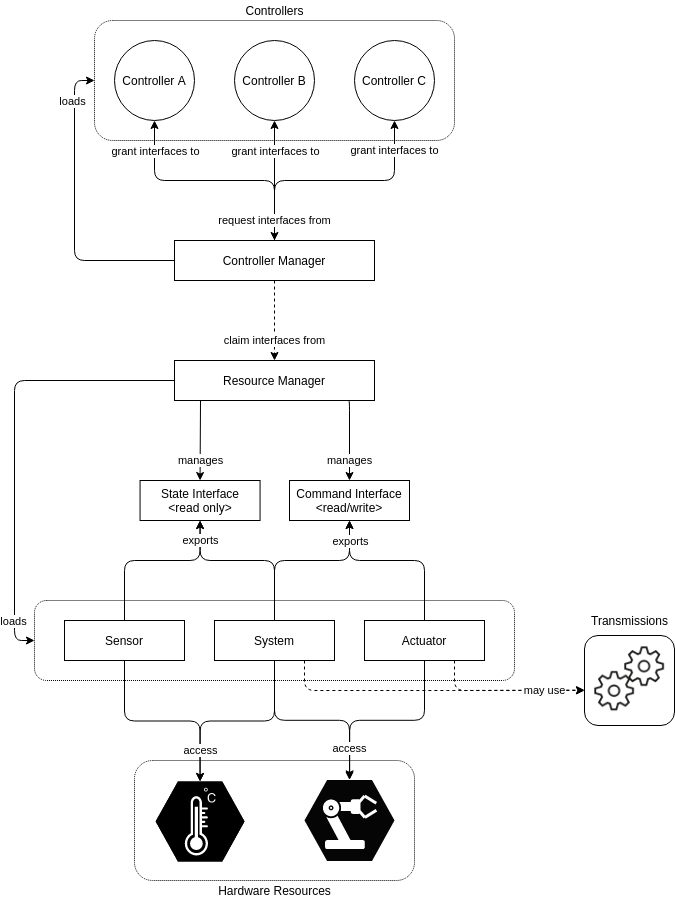
\includegraphics[width=120mm]{./fig/ros2_control/components_architecture.png}
  \vspace{2mm}
  \caption{ROS2 Control Framework. \cite{ros2control}}\label{ros2_control_framework}
\end{figure}

\subsubsection{ROS2 Control Overview}
The \texttt{ros2\_control} is a package providing a modular and configurable framework for controlling robotic systems. This package is a redevelopment of ros\_control \cite{ros_control}, used in ROS.

% In ros\_control, the rigid structure of \texttt{RobotHW} class and \texttt{CombinedRobotHardware} class \cite{ros_combined_robot_hw} are used for handling with hardware. Without any coding, this structure makes it difficult to extend additional hardware and sensor. In addition, to control the hardware, \texttt{position}, \texttt{velocity}, and \texttt{effort} are allowable.

% In ros2\_control framework, the plugins of hardware are divided into \texttt{Actuator}, \texttt{Sensor}, and \texttt{System}. Moreover, the type of hardware interface is not fixed. By the combination of these components, development of multi-robot and multi-sensor are available within this framework.

The ros\_control framework relies on the \texttt{RobotHW} class as a structure to manage hardware interactions. While it provides a rigid structure for handling various hardware components like sensors and actuators, extending existing robots with additional hardware requires coding, limiting the flexibility to integrate new elements. The use of the \texttt{CombinedRobotHardware} class \cite{ros_combined_robot_hw} attempts to address this limitation, yet it may not be optimal, especially when incorporating external sensors into the system.

In contrast, the ROS2 control framework introduces a more versatile approach by defining three types of hardware: \texttt{Actuator}, \texttt{Sensor}, and \texttt{System}. Through the composition of these basic components, any robotic cell, encompassing the robot and its surrounding environment, can be described. Unlike ros\_control, ros2\_control does not enforce a fixed set of interface types, allowing flexibility in defining interfaces. This ensures compatibility with standard controllers, as standard interfaces are defined as constants in the \texttt{hardware\_interface} package. Moreover, the \texttt{ControllerManager} in ros2\_control facilitates controlled access to the hardware by managing the state of available interfaces through the \texttt{ResourceManager}. Unlike ros\_control, controllers have no direct access to hardware, and they register their interfaces with the \texttt{ControllerManager}, enhancing modularity and resource conflict resolution.

% In Moonbot, each leg functions as an independent entity with its own controller, ensuring a high degree of modularity. This design choice aligns seamlessly with the modular structure of Moonbot, allowing for efficient control and adaptability across different leg configurations.

\subsubsection{Controller Manager}
At the heart of the ROS2 control architecture lies the Controller Manager. This component is responsible for loading, managing, and switching between different controllers. In Moonbot, the Controller Manager coordinates the operation of controllers associated with each leg, allowing dynamic transitions between various locomotion styles based on the robot's configuration.

\subsubsection{ROS2 Life Cycle}
ROS2 Lifecycle \cite{ros2lifecycle} is utilized in controller manager of ROS2 control. The ROS 2 Node Lifecycle provides enhanced control over the state of the ROS system, as shown in \fig{lifecycle}, ensuring the proper initualization of all components before executing any behavior. This mechanism enables nodes to be restarted or replaced while the system is running.

A key aspect emphasized in this document is the concept of a managed node, which adheres to a predefined interface and operates within a well-defined life cycle state machine. By treating managed nodes as black boxes, developers have flexibility in implementing the life cycle functionality while ensuring compatibility with management tools across all compliant nodes.\\

\begin{figure}[t]
  \centering
  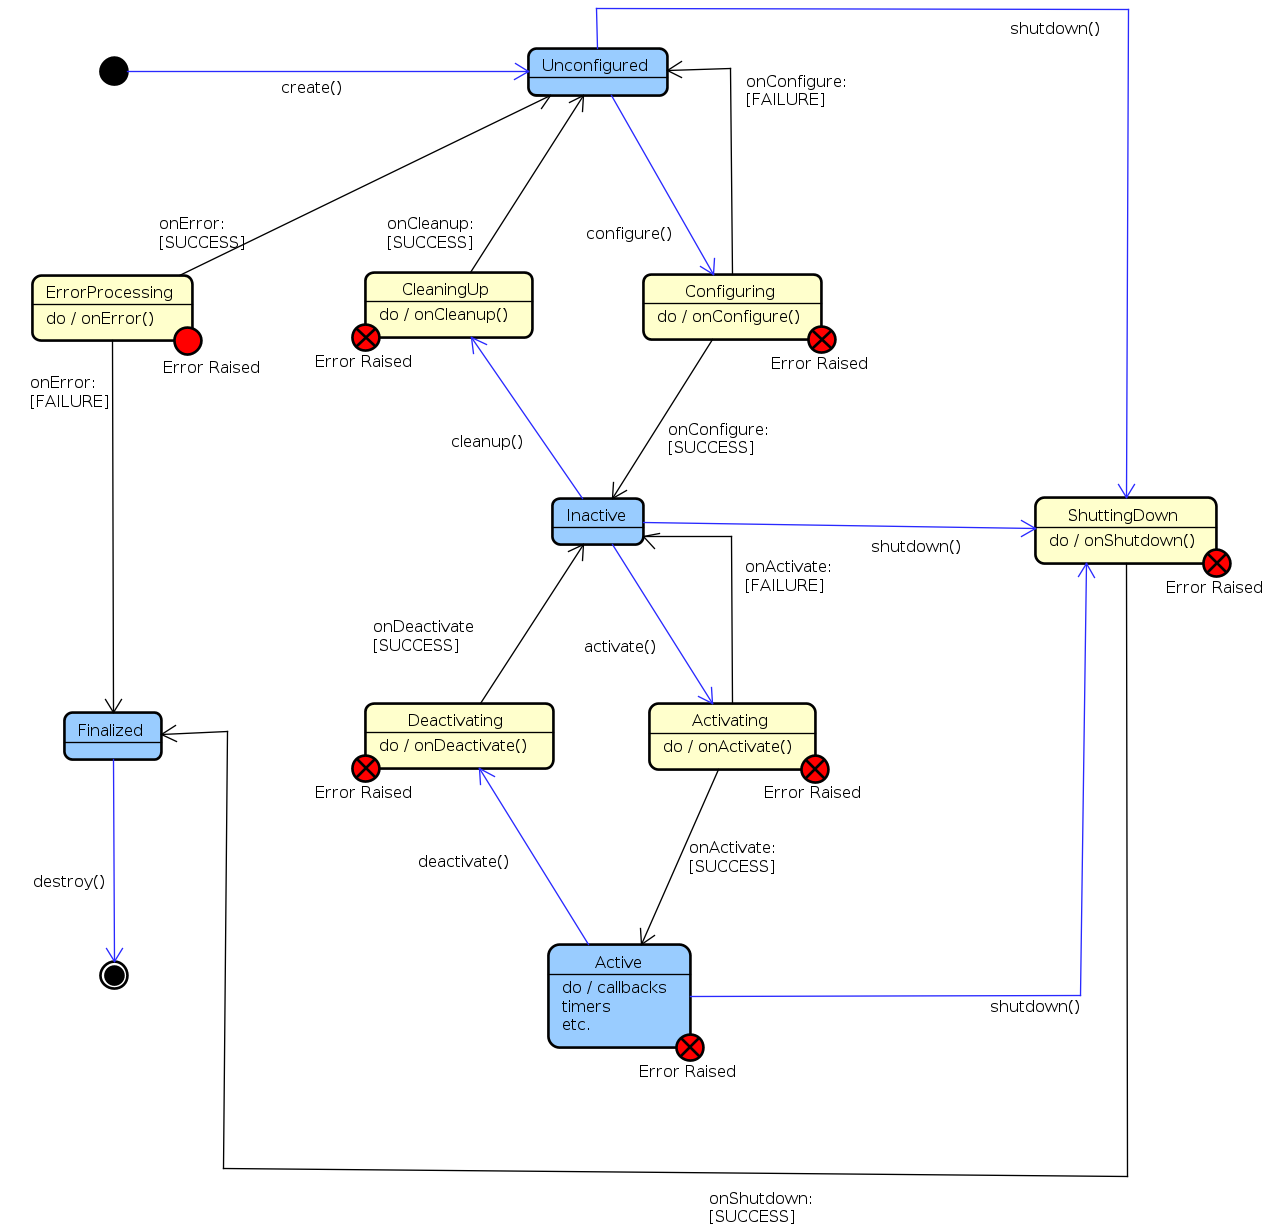
\includegraphics[width=\linewidth]{./fig/ros2_control/life_cycle_sm.png}
  \vspace{2mm}
  \caption{ROS2 Node Lifecycle. \cite{ros2lifecycle}}\label{lifecycle}
\end{figure}

\subsection{Dynamixel SDK \& Workbench}

\subsubsection{Dynamixel SDK}

The Dynamixel SDK (Software Development Kit) \cite{dynamixel-sdk} is a set of libraries and tools provided by ROBOTIS to interface with Dynamixel servos. It includes APIs (Application Programming Interfaces) for various programming languages such as C, C++, Python, and MATLAB, allowing developers to control Dynamixel servos easily from their preferred programming environment.

Key features of the Dynamixel SDK include:

\begin{itemize}
    \item \textbf{High-level APIs:} The SDK provides high-level APIs that abstract the low-level communication protocols of Dynamixel servos, making it easier for developers to control and interact with the servos.
    
    \item \textbf{Advanced control functionalities:} It offers advanced control functionalities such as position control, velocity control, torque control, and compliance control.
    
    \item \textbf{Diagnostic tools:} The SDK includes diagnostic tools that allow developers to monitor the status of Dynamixel servos, diagnose issues, and perform troubleshooting.
    
    \item \textbf{Community support:} ROBOTIS provides extensive documentation, tutorials, and forums to support developers using the Dynamixel SDK, fostering a vibrant community of users who share knowledge and resources.
\end{itemize}

\subsubsection{Dynamixel Workbench}
In addition to the Dynamixel SDK, ROBOTIS offers the Dynamixel Workbench \cite{dynamixel_workbench}, a higher-level software framework built on top of the SDK. Dynamixel Workbench provides a comprehensive set of tools and utilities for managing Dynamixel-based robotic systems. It includes features such as:

\begin{itemize}
    \item \textbf{Motion editing:} Dynamixel Workbench allows users to create and edit motion sequences for controlling Dynamixel servos in complex robotic behaviors.
    
    \item \textbf{Parameter tuning:} Users can adjust various parameters of Dynamixel servos, such as PID gains, compliance margins, and operational limits, to optimize performance and behavior.
    
    \item \textbf{Hardware interface:} Dynamixel Workbench includes APIs and drivers for interfacing with Dynamixel hardware, allowing users to communicate with servos, sensors, and other peripherals especially with ROS2 communication.
\end{itemize}

Together, the Dynamixel SDK and Dynamixel Workbench provide a powerful ecosystem for developing and controlling Dynamixel-based robotic systems, offering flexibility, scalability, and ease of use for researchers, educators, and hobbyists alike.

The Pinging function \cite{dynamixel_sdk_ping_protocol}, within Dynamixel SDK, serves as a fundamental component crucial for self-recognition algorithms in Moonbot. This function plays a pivotal role in enabling the system to identify and communicate with connected specific ID Dynamixel servos. By sending a ping command to each servo, the system can receive a response indicating the presence and status of the servos. This information is essential for initializing, configuring, and monitoring the servos within the robotic framework. 

%%%

\section{Self-Recognition}\label{HowToInsertLink}
In the context of our robotic system, self-recognition refers to the ability of the robot to autonomously assess the status and connectivity of its modules

Moonbot's adaptability is a cornerstone of its design, allowing for dynamic reconfiguration through the attachment and detachment of modules via magnetic connectors. To effectively control the robot, it is imperative for Moonbot to possess self-awareness regarding its current configuration and the type of connected module (e.g., yaw-pitch-pitch leg, gripper).

\subsection{Problem Statements}
\begin{enumerate}
    \item The robot need to be able to activate and deactivate the controller for any kinds of the module.

    \item With the different number of connected modules, the robot moves with different motion style.

\begin{figure}[h]
  \centering
  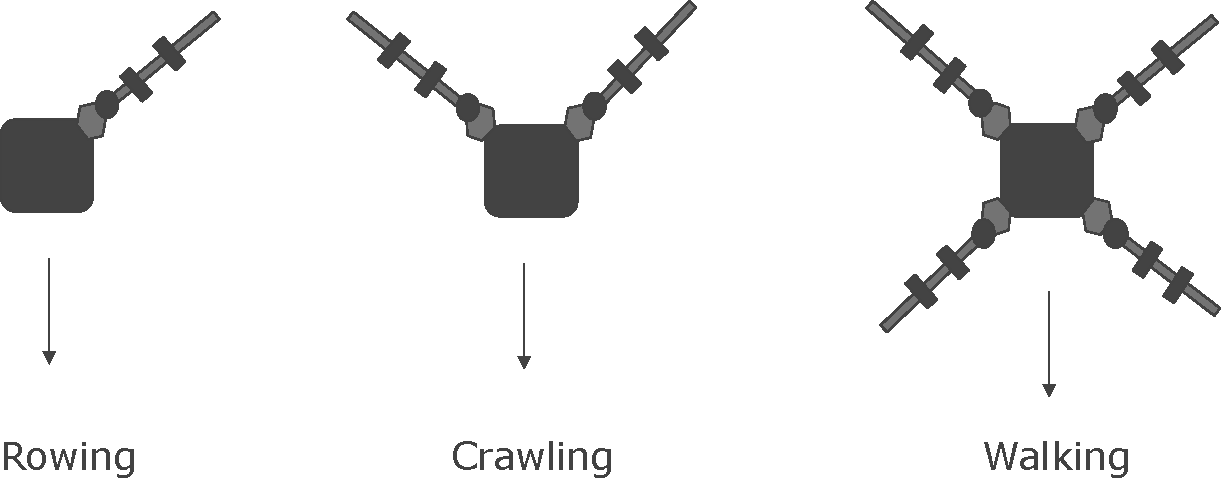
\includegraphics[width=110mm]{./fig/chap3/control_system/motion_selection.pdf}
  \vspace{2mm}
  \caption{Motion selection strategies for different number of module connections.}\label{motion_selection}
\end{figure}

    \item With the different kinds of module, the robot selects the proper motion for the specific module type.

\begin{figure}[h]
  \centering
   \rotatebox{90}{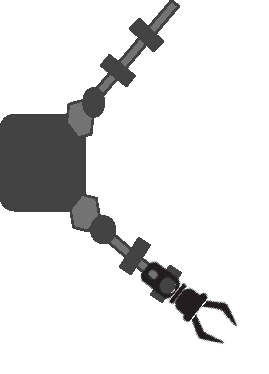
\includegraphics[width=35mm]{./fig/chap3/control_system/gripleg2.pdf}}
  \vspace{2mm}
  \caption{Different kind of modules connected to the robot.}\label{gripper}
\end{figure}
\end{enumerate}

\subsection{Algorithms Overview}
Inspired by the design of Snapbot, a modular-legged robot developed by Disney Inc. \cite{snapbot1}, \cite{snapbot2}, Moonbot employs a self-recognition system. The connections are periodically verified by pinging the specific ID of Dynamixel motors. The flowchart in \fig{flowchart} and Algorithm~\ref{alg:module_recognition} shows the modular connection algorithm for one connector. After the robot identifies the type of module, the module's controller at the specific port is independently launched, and activated. With the specific configuration identified, Moonbot then selects the appropriate locomotion style.
\vspace{1mm}

\begin{figure}[h]
  \centering
  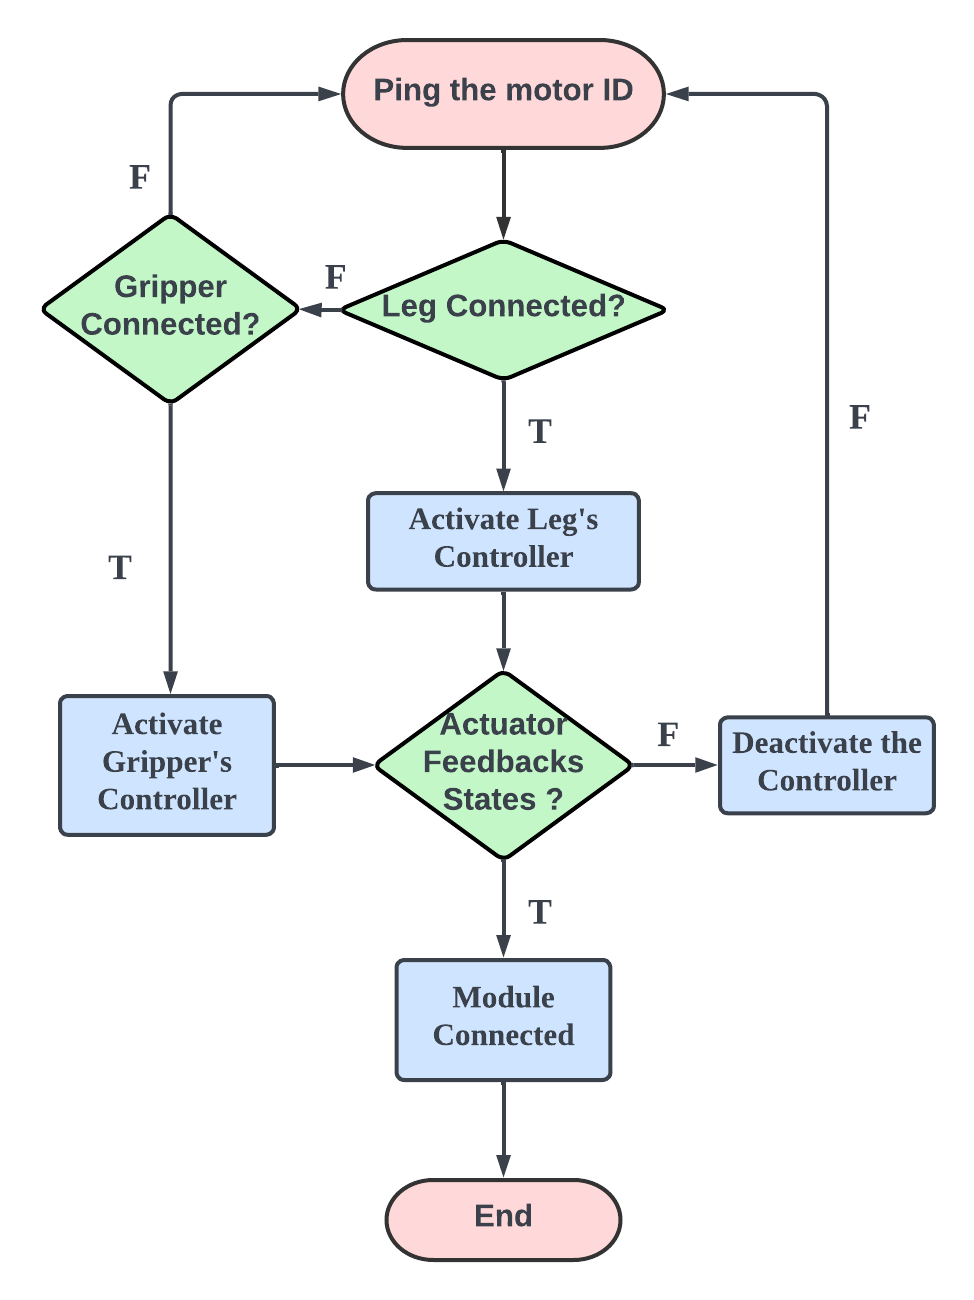
\includegraphics[width=90mm]{./fig/flowchart/flowchartcolor.png}
  \vspace{2mm}
  \caption{Self-recognition algorithm for each connection.}\label{flowchart}
\end{figure}

\begin{algorithm}[h]
\caption{Self-Recognition for module connection at right-rear port.}
\label{alg:module_recognition}
\begin{algorithmic}[1]
\Function{RR\_initializer\_callback}{}
    
    \If{\texttt{no RR\_module\_detected}}
        \If{\texttt{Found leg module at RR port}}
            \State \texttt{Activate leg's controller at RR port}
            % \State \texttt{RR\_detected = True}
            % \State \texttt{RR\_leg\_connected = True}
        \ElsIf{\texttt{Found gripper module at RR port}}
            \State \texttt{Activate gripper's controller at RR port}
            % \State \texttt{self.RR\_detected = True}
            % \State \texttt{self.RR\_gripper\_connected = True}
        % \Else
        %     \State \texttt{`No RR state detected!'}
        \EndIf
        
    \ElsIf{\texttt{RR\_module\_detected}}
        \If{\texttt{RR\_leg\_connected}}
            \If{\texttt{RR\_state error}}
                \State \texttt{Deactivate leg's controller at RR}
                % \State \texttt{RR\_leg\_connected = False}
                % \State \texttt{RR\_detected = False}
            % \Else
            %     \State \texttt{`RR CONNECTED!'}
            %     \State \texttt{RR\_detected = True}
            \EndIf
            
        \ElsIf{\texttt{RR\_gripper\_connected}}
            \If{\texttt{RR\_state error}}
                \State \texttt{Deactivate gripper's controller at RR}
                % \State \texttt{RR\_gripper\_connected = False}
                % \State \texttt{RR\_detected = False}
            % \Else
            %     \State \texttt{self.get\_logger().info(f"RR CONNECTED!")}
            %     \State \texttt{self.RR\_detected = True}
            \EndIf
        \EndIf
    \EndIf
\EndFunction
\end{algorithmic}
\end{algorithm}

\subsection{Node Structure and Components}
The controller of the Moonbot are separated for each connector, including limbs—RF (Right Front), LF (Left Front), LR (Left Rear), and RR (Right Rear) as shown in \fig{mb_control}. From this structure, to control the motion, four launching services are needed to be implemented for each controller. With the framework of ROS2 control, we can handled the command and state of each joint independently. Consequently, the module detection node handle the joint states of four specific ports, separately. \\
% \vspace{5mm}

\begin{figure}[h]
  \centering
  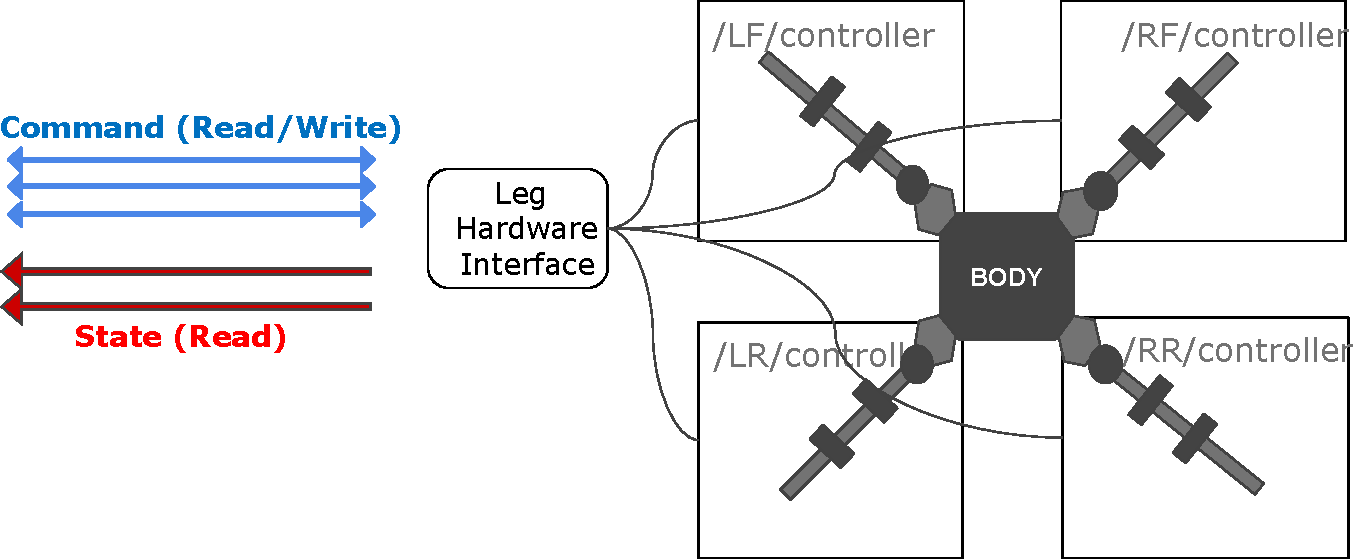
\includegraphics[width=140mm]{./fig/chap3/control_system/mb_control2.pdf}
  \vspace{2mm}
  \caption{Separated controller for each module.}\label{mb_control}
\end{figure}

% \subsection{Flowchart \& Algorithms}


\subsection{Initialization Process}
The initialization process is involved with activation of the controller into the life cycle of control, as we have discussed in the section of controller manager.

Upon initiation, the nodes for module detection check the availability of the corresponding hardware by attempting to communicate with the actuators (pinging). The communication is established through Dynamixel motors with the specific ID number. After the success of this communication, the module detection node sends the request to the service server that handle the launch service of actuator activation.  

% In addition, the state of the motors is the key parameter for monitoring the existence of module connection.

\subsection{Periodic Connection Status Monitoring}
% Following the initialization, the node continuously monitors the joint states of each module at regular intervals. The joint states provide information about the current position of the limbs' joints. This periodic monitoring is facilitated by timer callbacks dedicated to each limb. 

% In addition, the motors status monitoring also functions as a error detector. If the joint position of a limb deviates beyond a predefined threshold, which occurs when the motors is not connected and the states are unreadable, it indicates a potential issue such as disconnection or misalignment. In such cases, the node dynamically updates the connection status for that module.

% Unfortunately, the current version of \textit{hardware\_interface} in ROS2 control has not been implemented with the restart function feature for lost hardware yet. Therefore, the launch services contain the function to automatically shutdown the process of controller manager which means disconnection the hardware from the software control. If the hardware is reconnected to the connector and is detected, the program operates the same process as the initialization and relaunch the activity of ROS2 control again.

Following the initialization, the node continuously monitors the joint states of each module at regular intervals, providing real-time information on the current position of the limbs' joints. Timer callbacks dedicated to each limb facilitate this periodic monitoring.

Additionally, the node functions as an error detector by monitoring the status of the motors. If a joint position deviates beyond a predefined threshold, indicating potential issues like disconnection or misalignment, the node dynamically updates the connection status for that module.

However, it's worth noting that the current version of the \textit{hardware\_interface} in ROS2 control does not include a restart function for lost hardware. Therefore, the launch services incorporate a feature to automatically shut down the controller manager process in response to hardware disconnection. Upon reconnecting the hardware, the program reinitializes the ROS2 control activity, relaunching the controller manager process.

\subsection{Adaptability to Grippers}
The Dynamixel motors offer a unique ID identification feature, accessible through the Dynamixel Wizard GUI tool \cite{dynamixel_wizard2}, which facilitates initial setup. In Moonbot's control system, the module detection node is designed to identify specialized components, such as grippers, by searching for specific motor IDs. For instance, a motor ID of 1 corresponds to the leg module, while an ID of 2 signifies the gripper module. By extending self-recognition capabilities to include end-effectors, we enhance the versatility of our robotic system.\\

\begin{figure}[h]
  \centering
  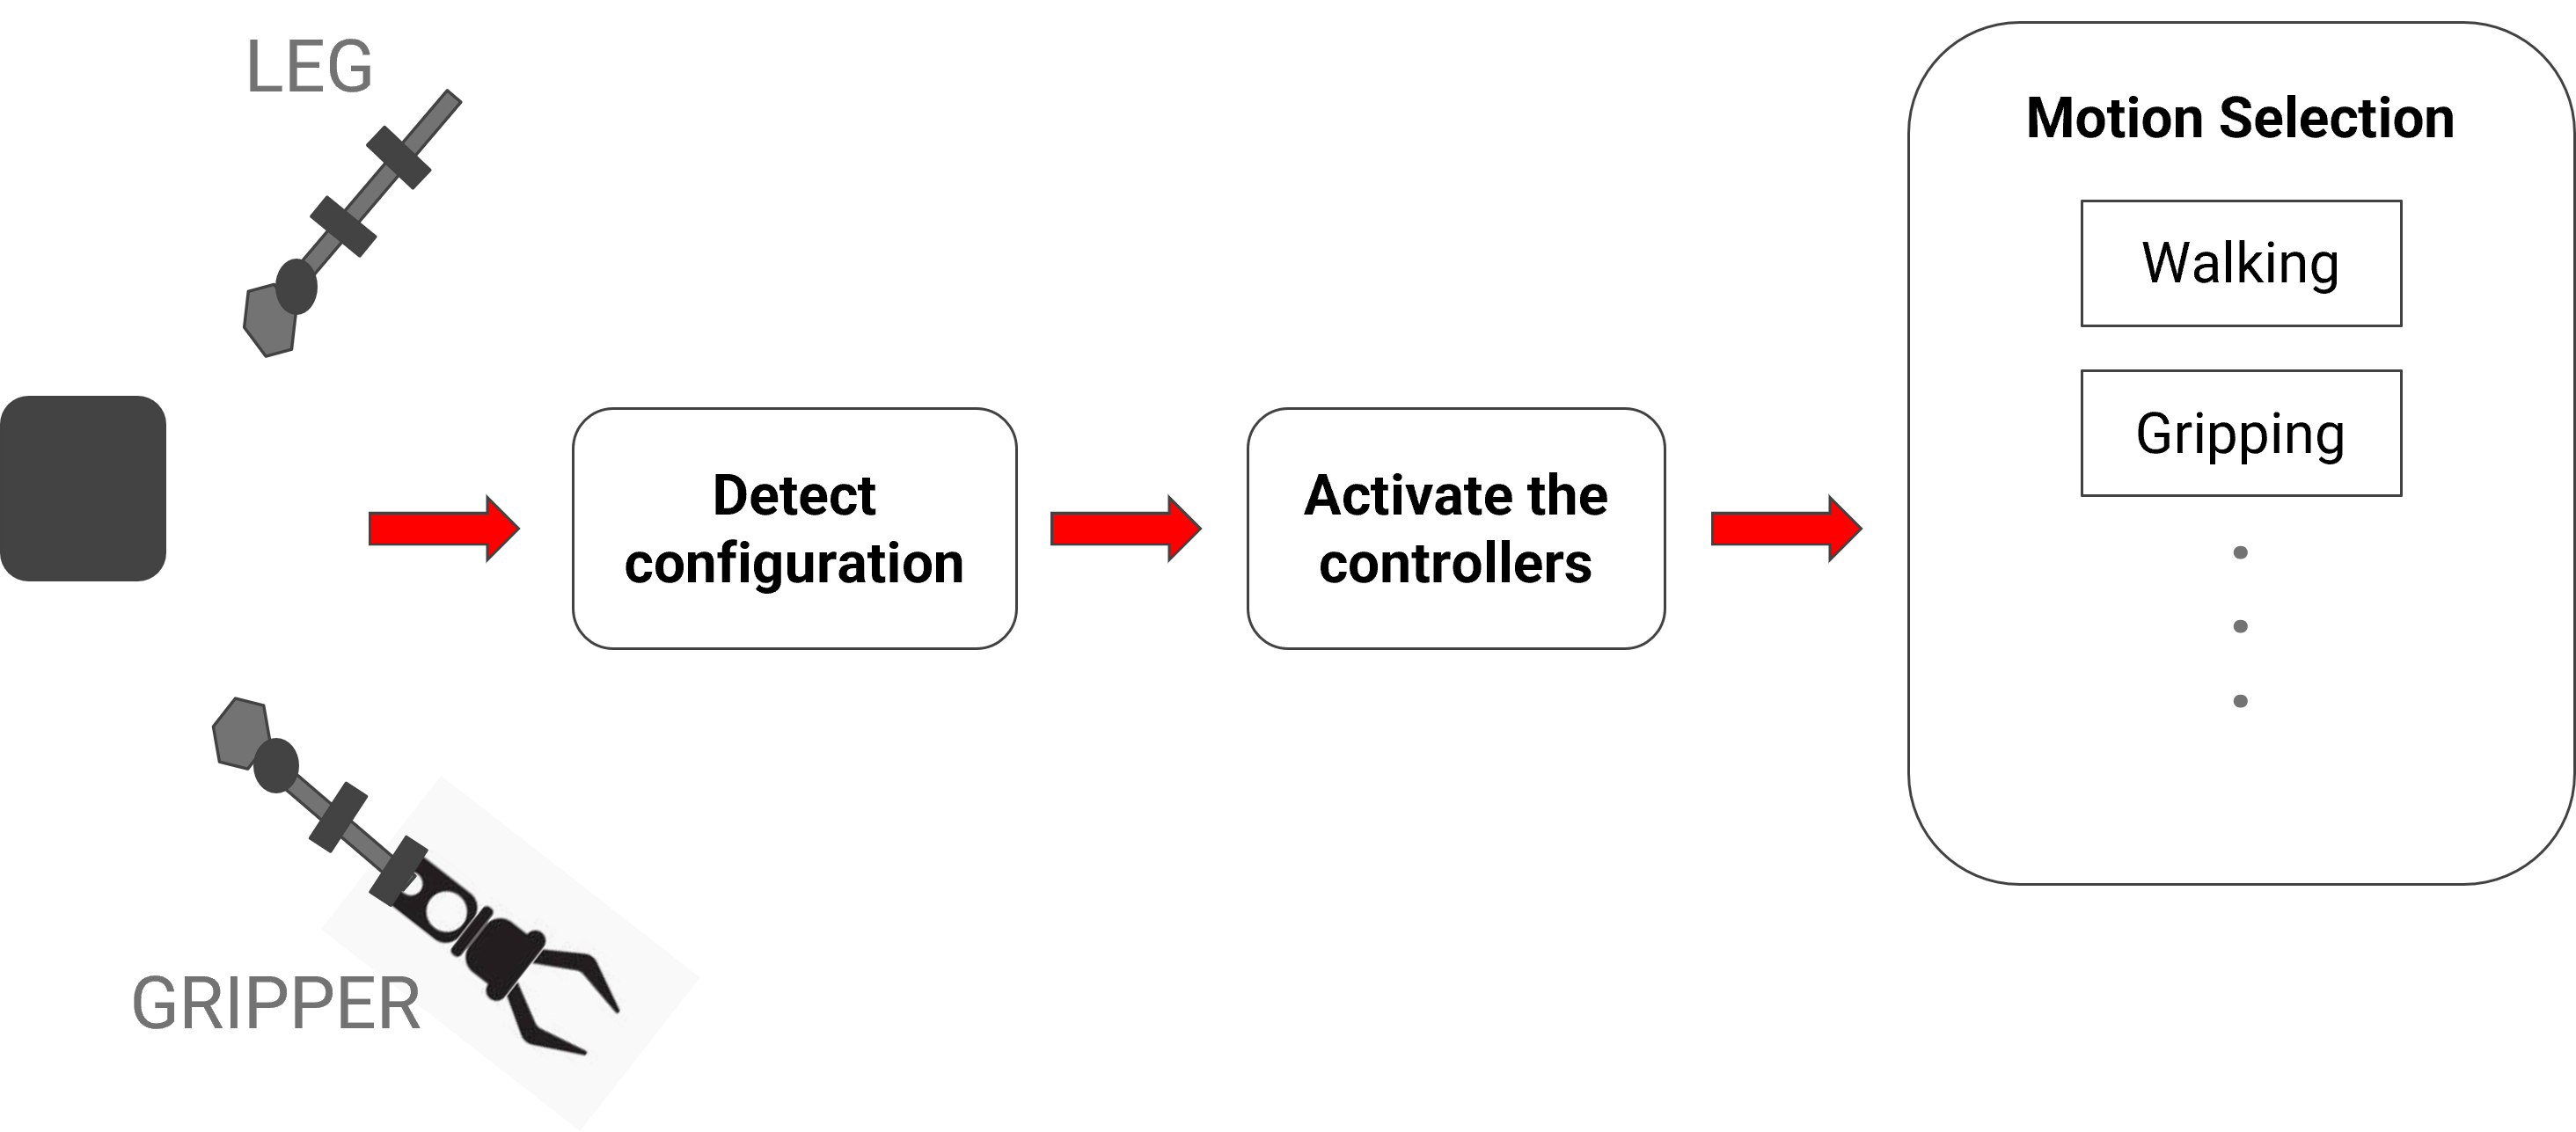
\includegraphics[width=130mm]{./fig/chap3/control_system/leggrip.png}
  \vspace{2mm}
  \caption{Motion selection depending on module type.}\label{gripleg}
\end{figure}

\subsection{Motion Selection}
After the implementation of connection recognition of the module is success, the self-recognition algorithm can report the connection status of each connector in real-time, periodically. From this information, we can perform an experiment for motion selection depending on Moonbot configuration's which are mentioned in the problem statements.

To present the adaptability of the modular legged robot, Moonbot's locomotion styles including crawling motion and walking motion. The motion style is selected by the number of leg module connection.

\label{enumerate}
\begin{enumerate}
\item \textit{Crawling Motion:}
Moonbot moves by crawling motion when operating with a single-leg configuration towards the direction of connected module. Extending its capabilities, two-legged and three-legged configuration, Moonbot move with the same style as single configuration, but higher power by more legs applied.\\


\begin{figure}[h]
  \centering
  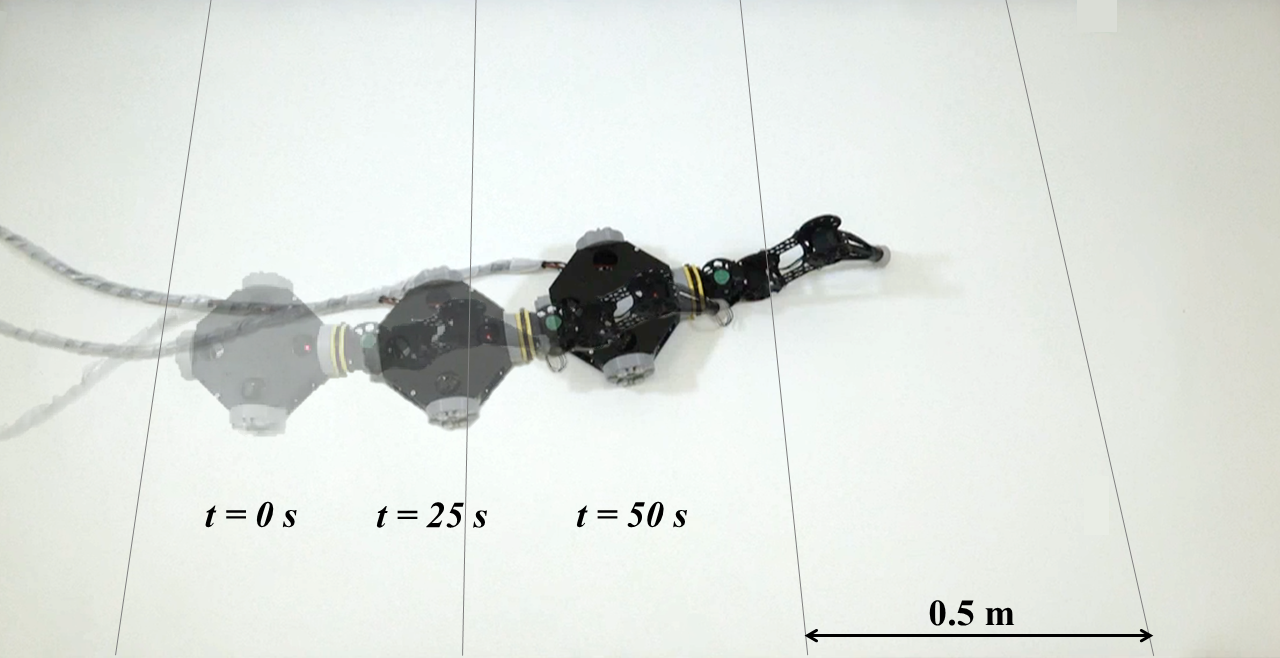
\includegraphics[width=110mm]{./fig/chap3/snapshot/single_snapshot4.png}
  \vspace{2mm}
  \caption{Snapshots of crawling motion for single-leg configuration.}\label{singlesnap}
\end{figure}


% \begin{figure}[h]
%   \centering
%   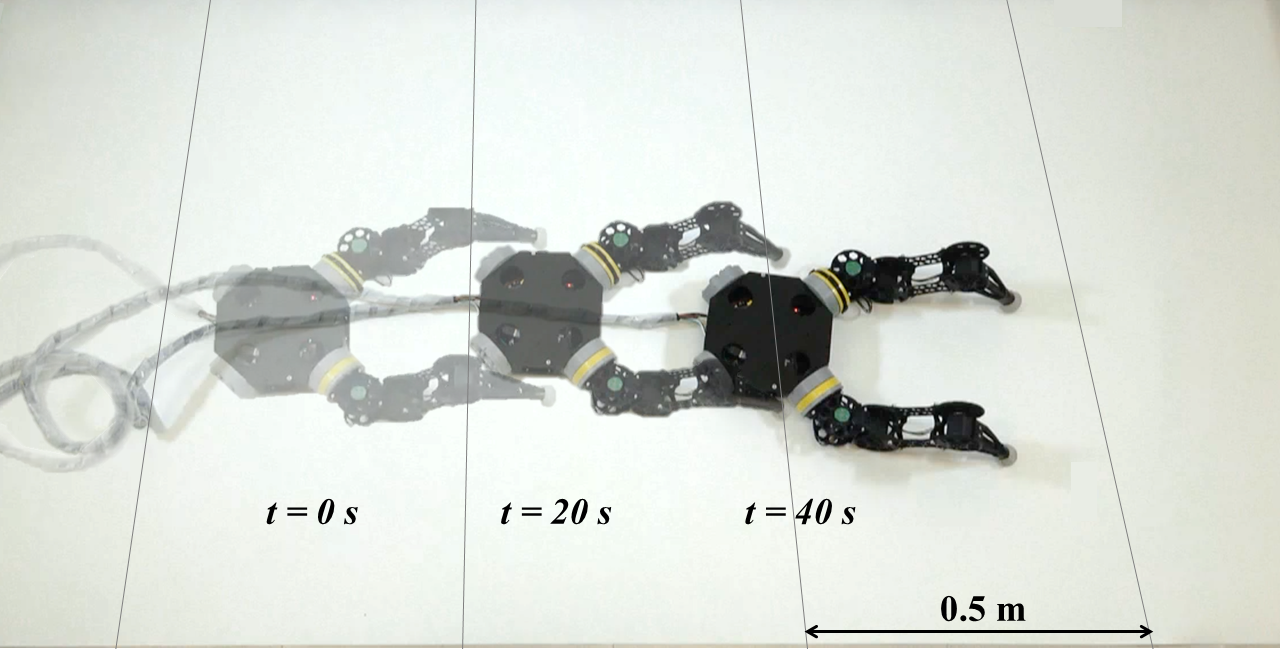
\includegraphics[width=110mm]{./fig/chap3/snapshot/double_snapshot3.png}
%   \vspace{2mm}
%   \caption{Snapshots of crawling motion for double-leg configuration.}\label{doublesnap}
% \end{figure}

% \begin{figure}[h]
%   \centering
%   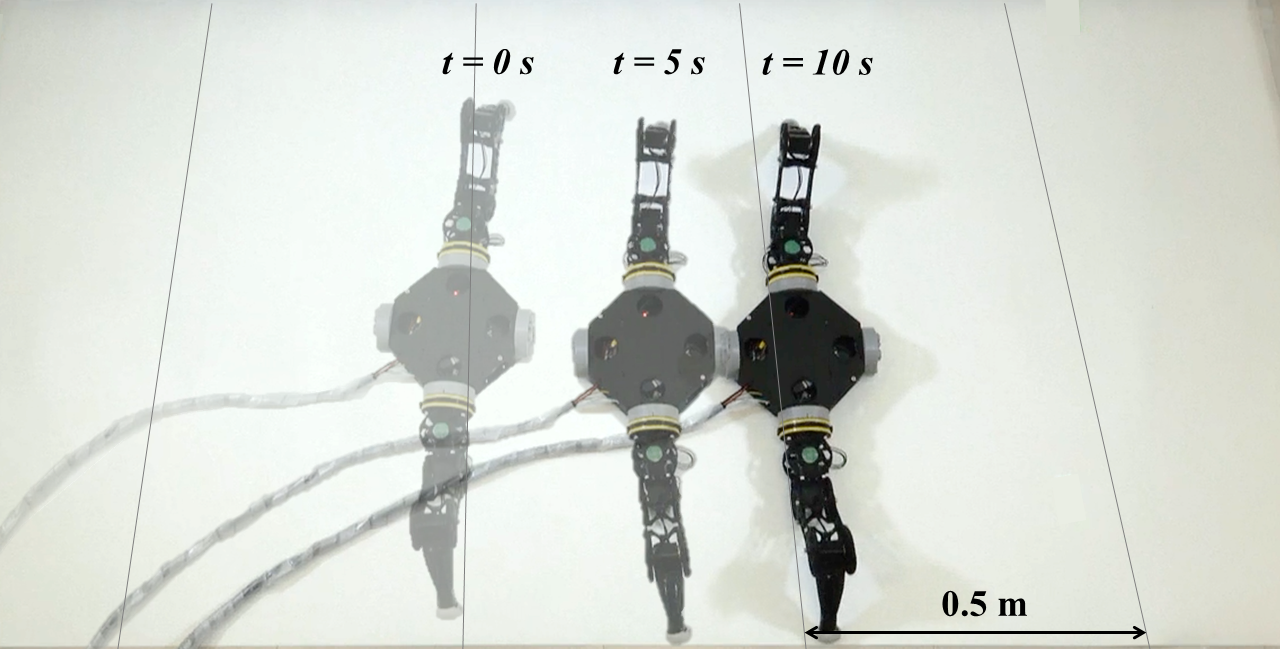
\includegraphics[width=110mm]{./fig/chap3/snapshot/double_snapshot4.png}
%   \vspace{2mm}
%   \caption{Snapshots of crawling motion for double-leg at opposite ports configuration.}\label{doublesnap2}
% \end{figure}

\begin{figure}[h]
 \begin{subfigure}{1.0\textwidth}
 \begin{center}
  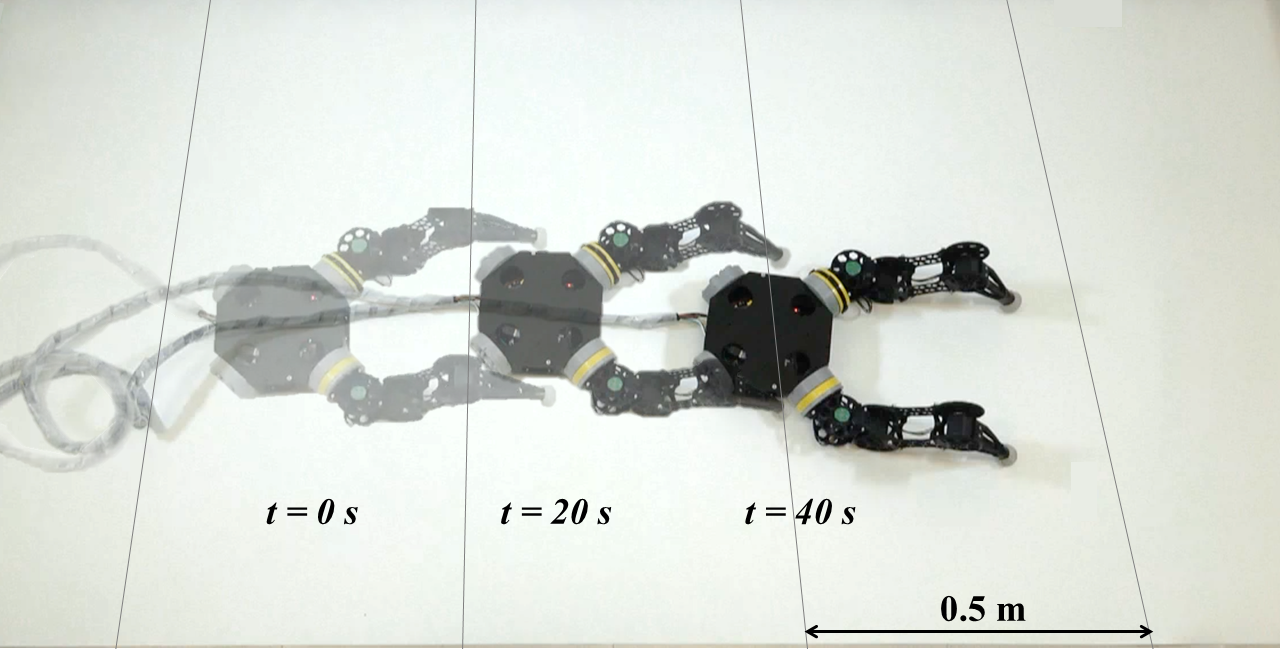
\includegraphics[width=110mm]{./fig/chap3/snapshot/double_snapshot3.png}
% \vspace{2mm}
  \caption{Crawling motion for double-leg configuration.}\label{doublesnap1}
 \end{center}
 \end{subfigure}
 
 \begin{subfigure}{1.0\textwidth}
 \begin{center}
  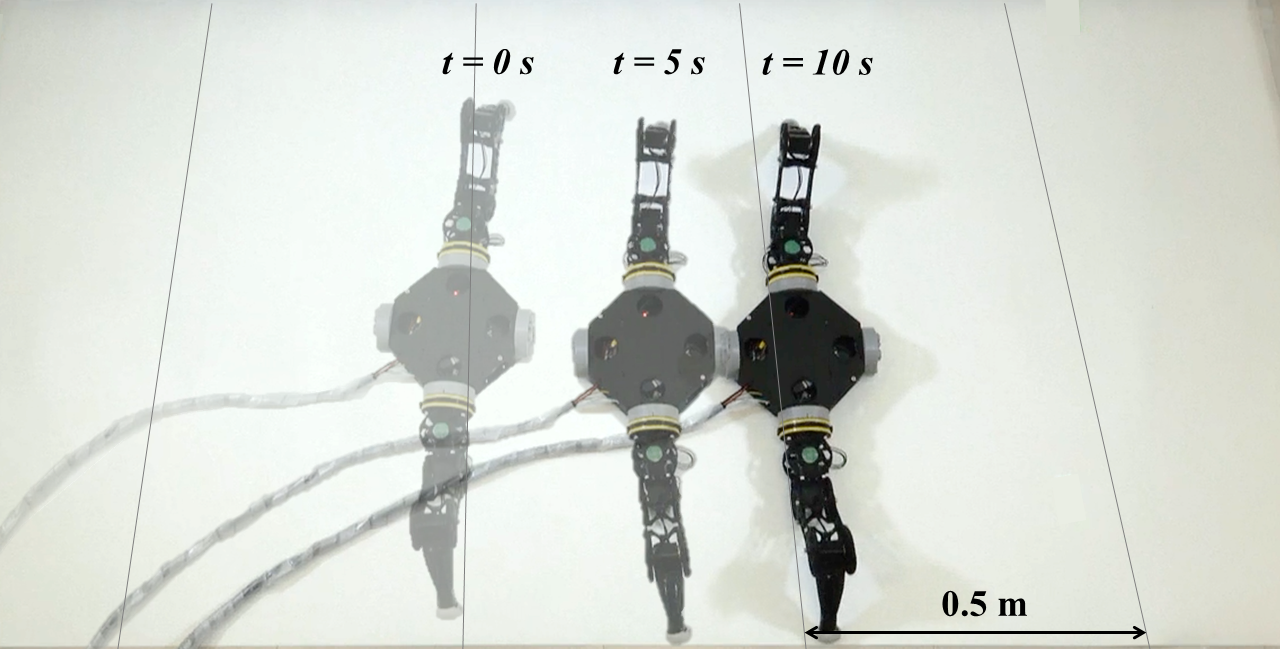
\includegraphics[width=110mm]{./fig/chap3/snapshot/double_snapshot4.png}
% \vspace{2mm}
  \caption{Crawling motion for double-leg at opposite ports configuration.}\label{doublesnap2}
\end{center}
\end{subfigure}
\vspace{-2mm}
\caption{Snapshots of crawling motion for double-leg configuration.}
\label{doublesnap}
\end{figure}




% \begin{figure}[h]
%  \centering
%  \begin{subfigure}{0.2\textwidth}
%  \begin{center}
%   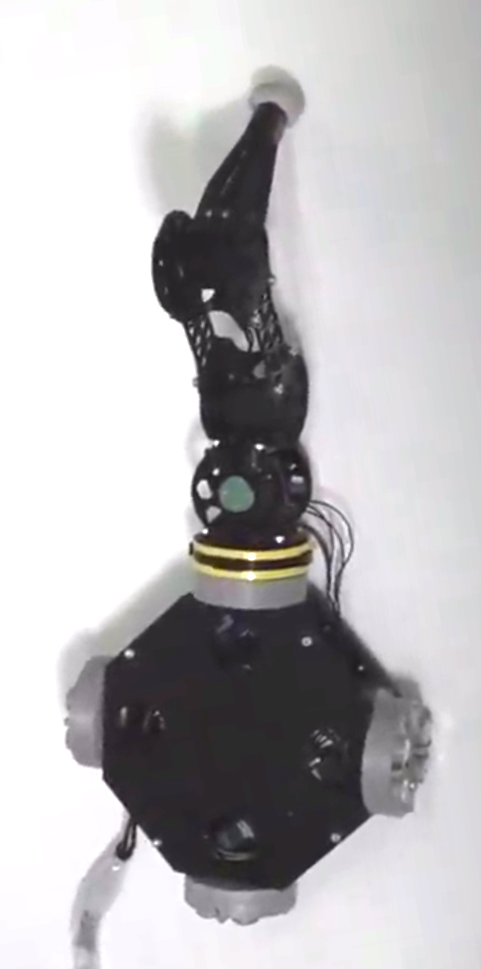
\includegraphics[width=25mm]{./fig/locomotion/11.png}
% \caption{Neutral pose}\label{snapshot1.1}
%  \end{center}
%  \end{subfigure}
%  \begin{subfigure}{0.2\textwidth}
%  \begin{center}
%   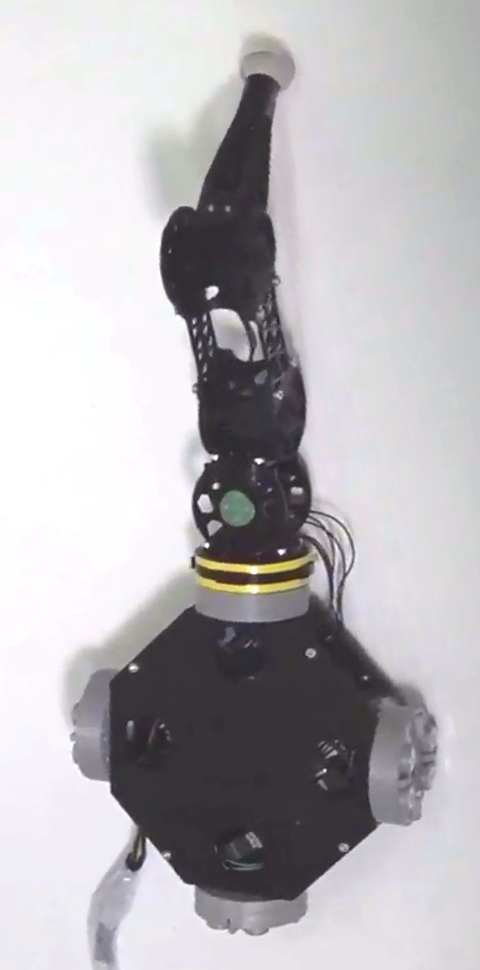
\includegraphics[width=25mm]{./fig/locomotion/12.png}
% \caption{Stretch the leg}\label{snapshot1.2}
% \end{center}
% \end{subfigure}
%  \begin{subfigure}{0.2\textwidth}
%  \begin{center}
%   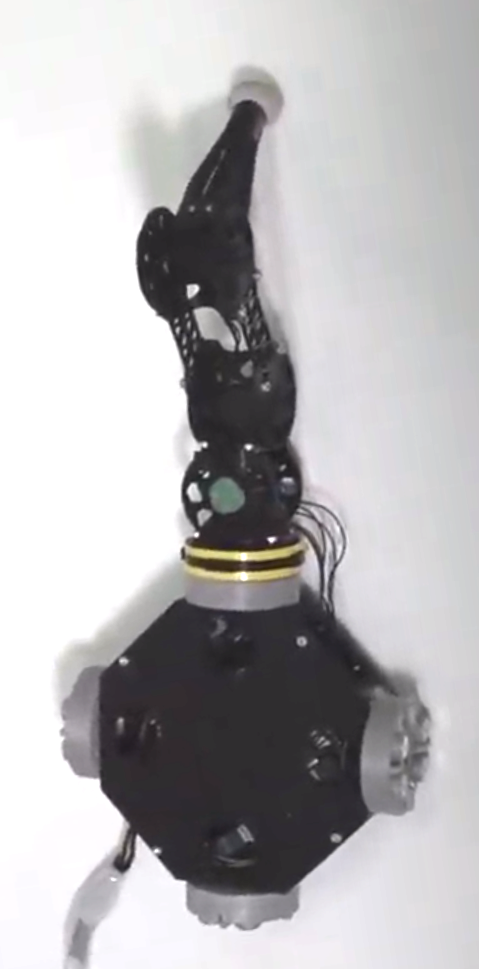
\includegraphics[width=25mm]{./fig/locomotion/13.png}
% \caption{Pulling forward}\label{snapshot1.3}
%  \end{center}
%  \end{subfigure}
% \vspace{-1mm}
% \caption{Crawling motion for single-leg configuration}
% \label{snap1}
% \end{figure}

% \begin{figure}[h]
%  \centering
%  \begin{subfigure}{0.2\textwidth}
%  \begin{center}
%   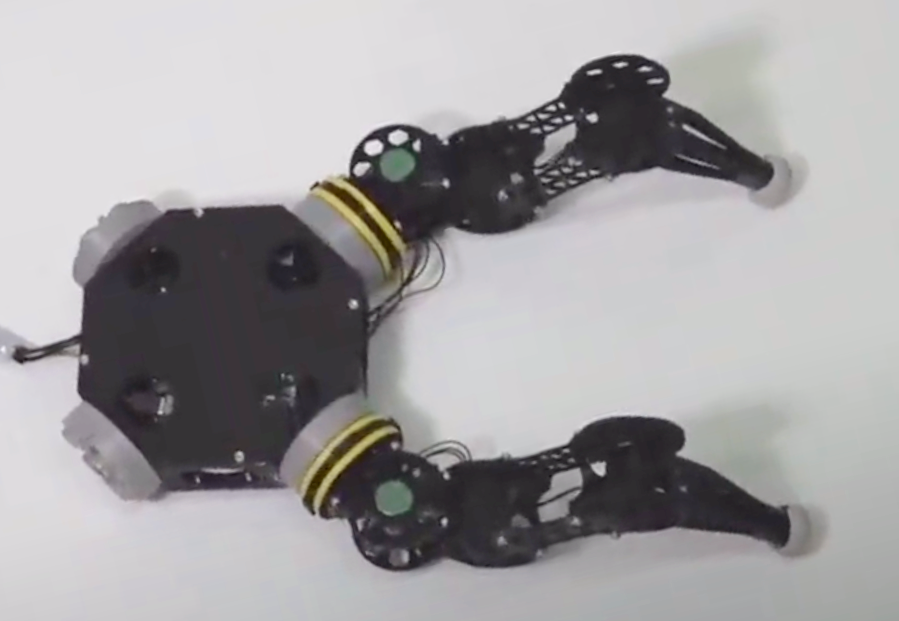
\includegraphics[width=40mm, angle=90]{./fig/locomotion/21.png}
% \caption{Neutral pose}\label{snapshot2.1}
%  \end{center}
%  \end{subfigure}
%  \begin{subfigure}{0.2\textwidth}
%  \begin{center}
%   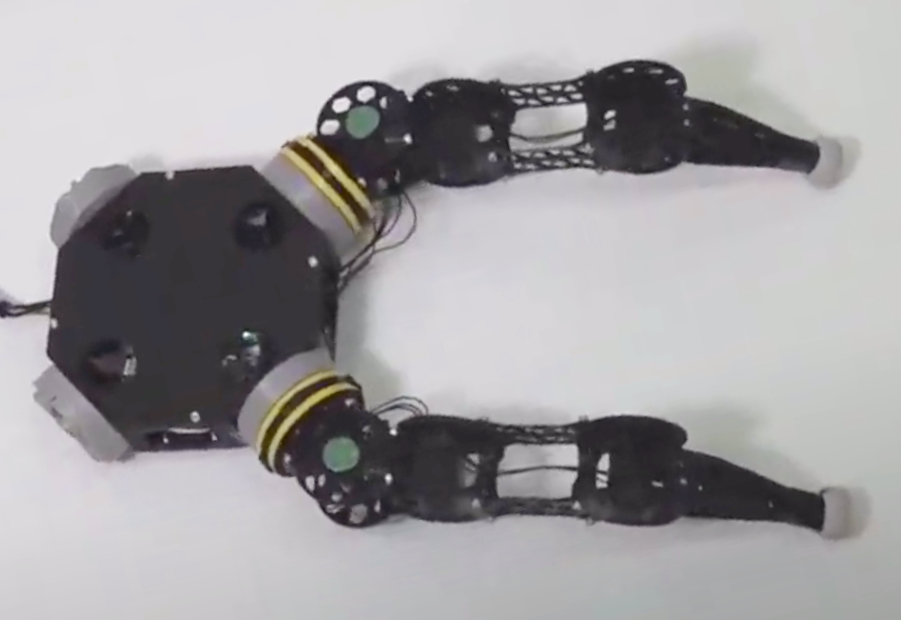
\includegraphics[width=40mm, angle=90]{./fig/locomotion/22.png}
% \caption{Stretch the leg}\label{snapshot2.2}
% \end{center}
% \end{subfigure}
%  \begin{subfigure}{0.2\textwidth}
%  \begin{center}
%   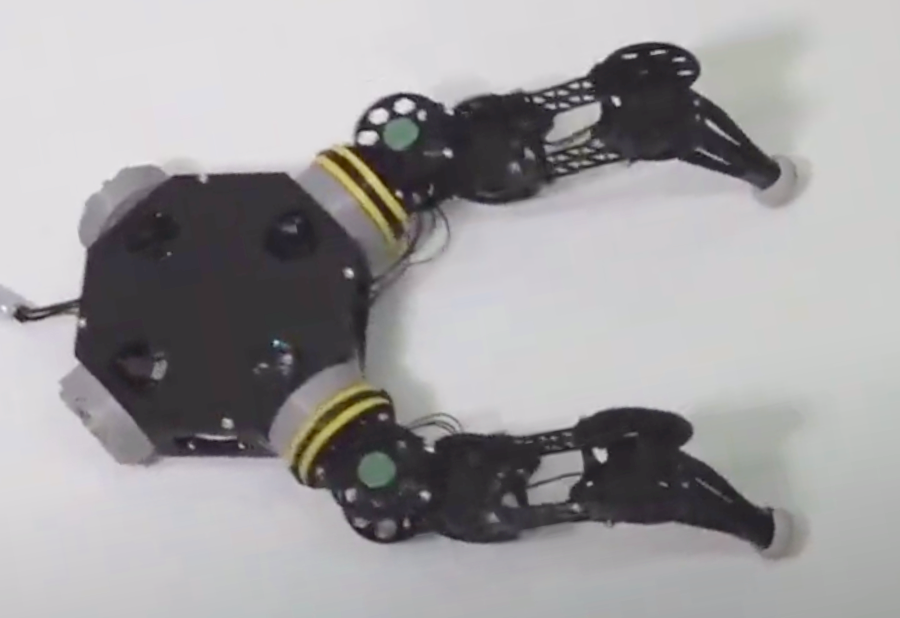
\includegraphics[width=40mm, angle=90]{./fig/locomotion/23.png}
% \caption{Pulling forward}\label{snapshot2.3}
%  \end{center}
%  \end{subfigure}
% % \vspace{-1mm}
% \caption{Crawling motion for double-leg configuration}
% \label{snap2}
% \end{figure}



\item \textit {Walking motion:}
In full configuration, employing all four legs, is designed for versatile locomotion. Moonbot can perform both a crawl gait for static stability and a trot gait for a more dynamic walking motion. \\
% \begin{itemize}
%     \item \textbf{Crawl gait}: Provides static stability by moving one or more legs at a time while maintaining contact with the ground. This gait is well-suited for navigating rough or uneven terrain where stability is crucial.

%     \item \textbf{Trot gait}: Offers a more dynamic walking motion by coordinating the movement of diagonally opposite legs. This gait allows for faster locomotion and is suitable for traversing relatively flat or open terrain.
% \end{itemize}

\begin{figure}[h]
  \centering
  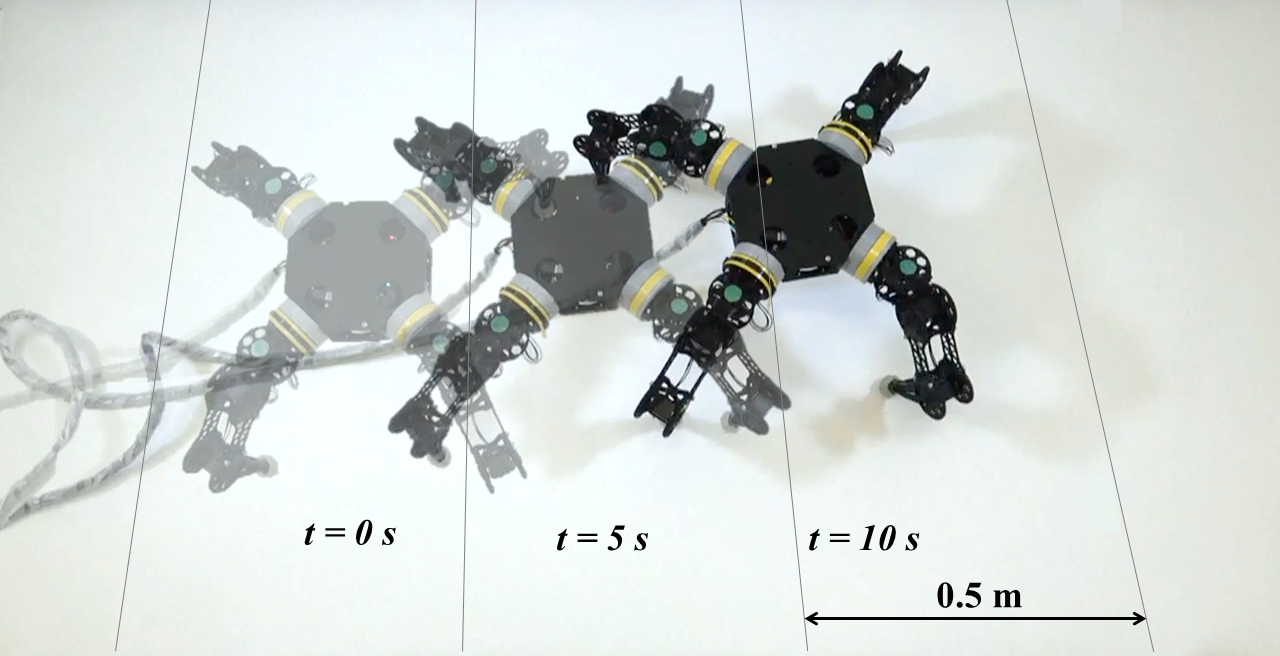
\includegraphics[width=110mm]{./fig/chap3/snapshot/full_snapshot4.png}
  \vspace{2mm}
  \caption{Snapshots of walking motion in self-recognition test.}\label{fullsnap}
\end{figure}

%%%
% \begin{figure}[h]
%   \centering
%   \begin{minipage}[ht]{0.2\textwidth}
%     \centering
%     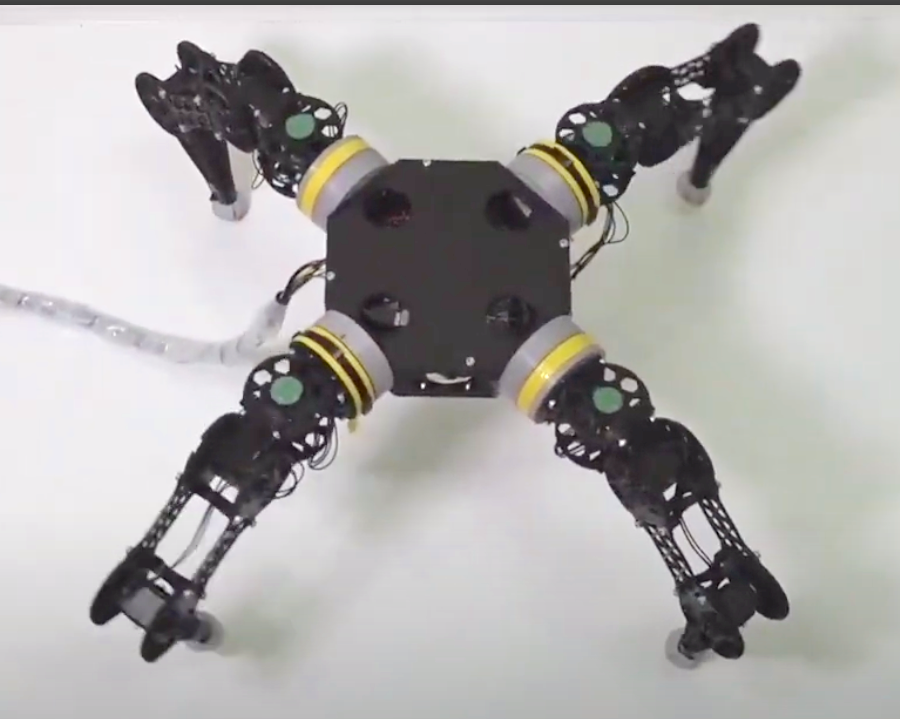
\includegraphics[clip, width=30mm]{./fig/locomotion/40.png}
%   \end{minipage}
%   \begin{minipage}[ht]{0.2\textwidth}
%     \centering
%     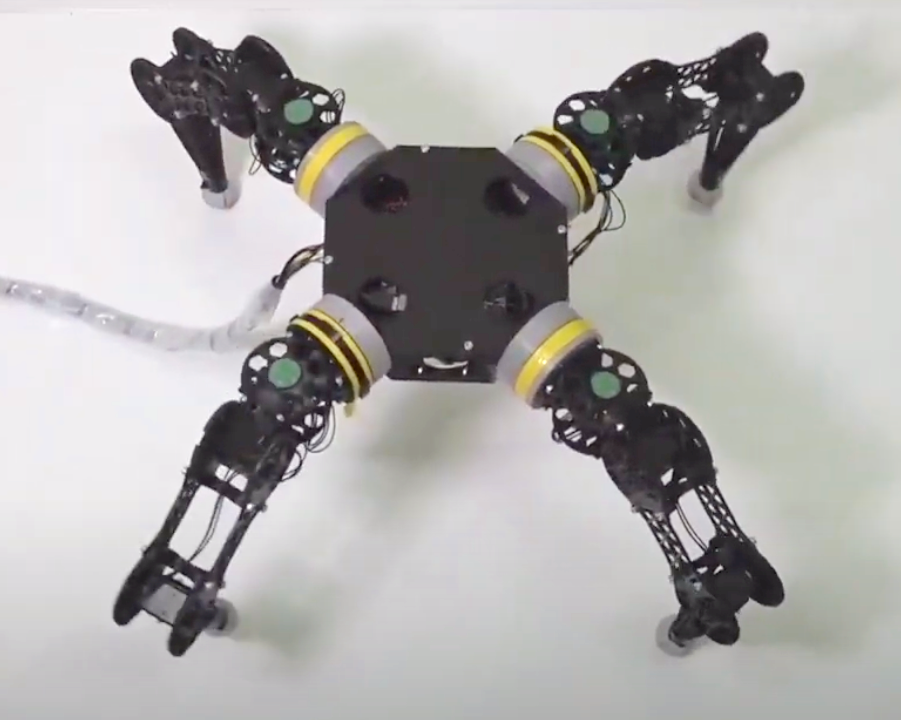
\includegraphics[clip, width=30mm]{./fig/locomotion/41.png}
%   \end{minipage}
%   \begin{minipage}[ht]{0.2\textwidth}
%     \centering
%     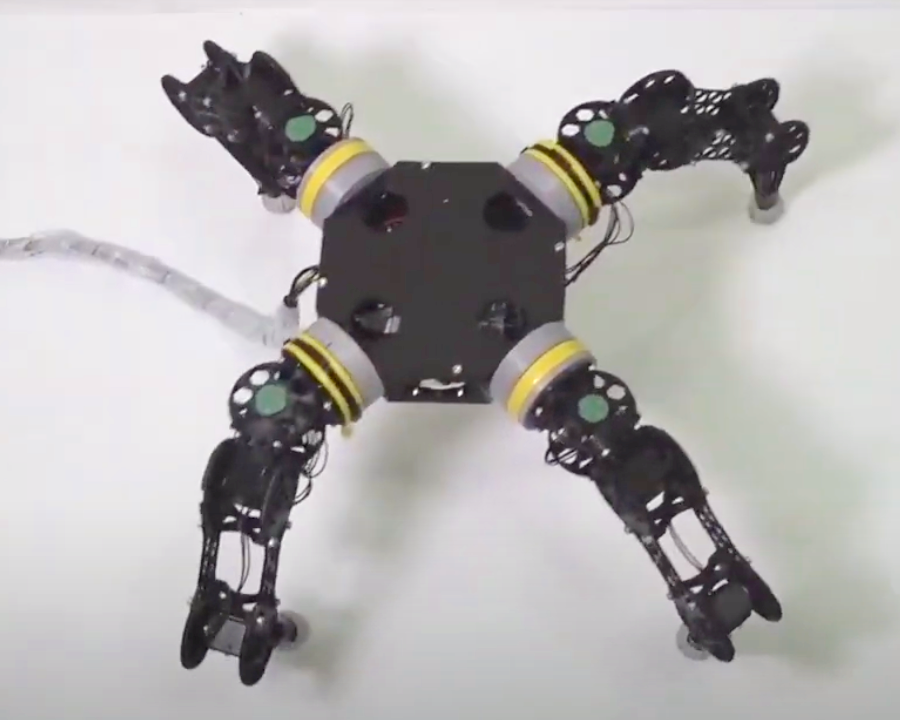
\includegraphics[clip, width=30mm]{./fig/locomotion/42.png}
%   \end{minipage}
%   \begin{minipage}[ht]{0.2\textwidth}
%     \centering
%     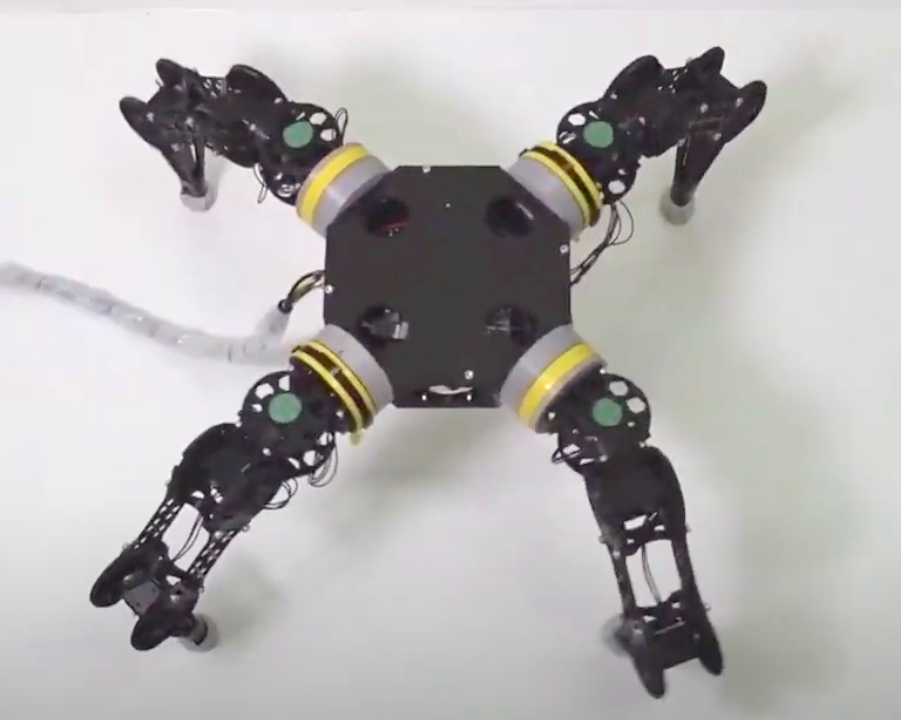
\includegraphics[clip, width=30mm]{./fig/locomotion/43.png}
%   \end{minipage}\\
%   \begin{minipage}[ht]{0.2\textwidth}
%     \centering
%     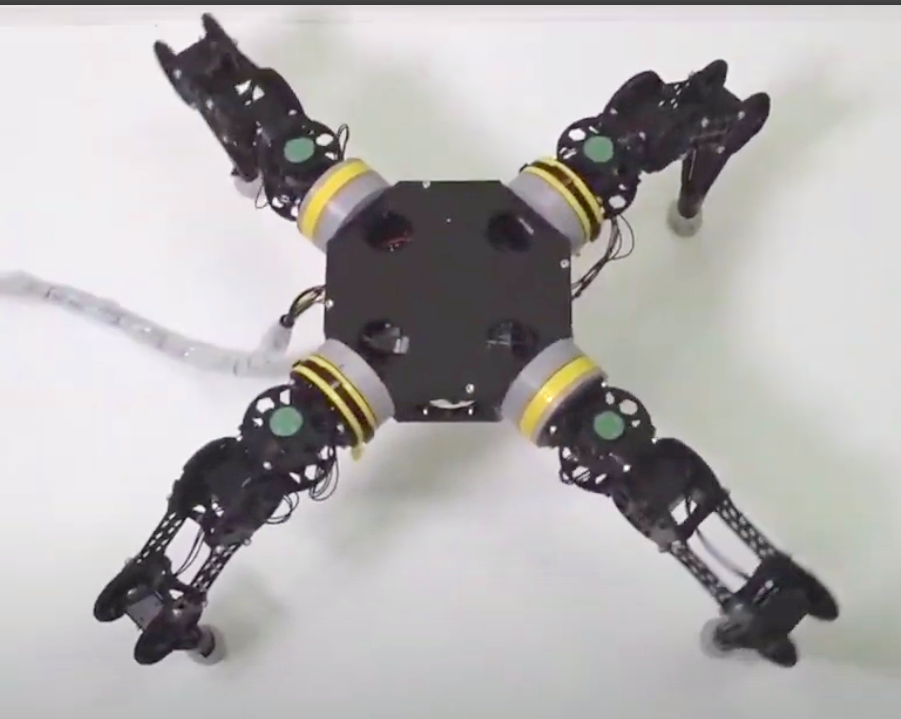
\includegraphics[clip, width=30mm]{./fig/locomotion/44.png}
%   \end{minipage}
%   \begin{minipage}[ht]{0.2\textwidth}
%     \centering
%     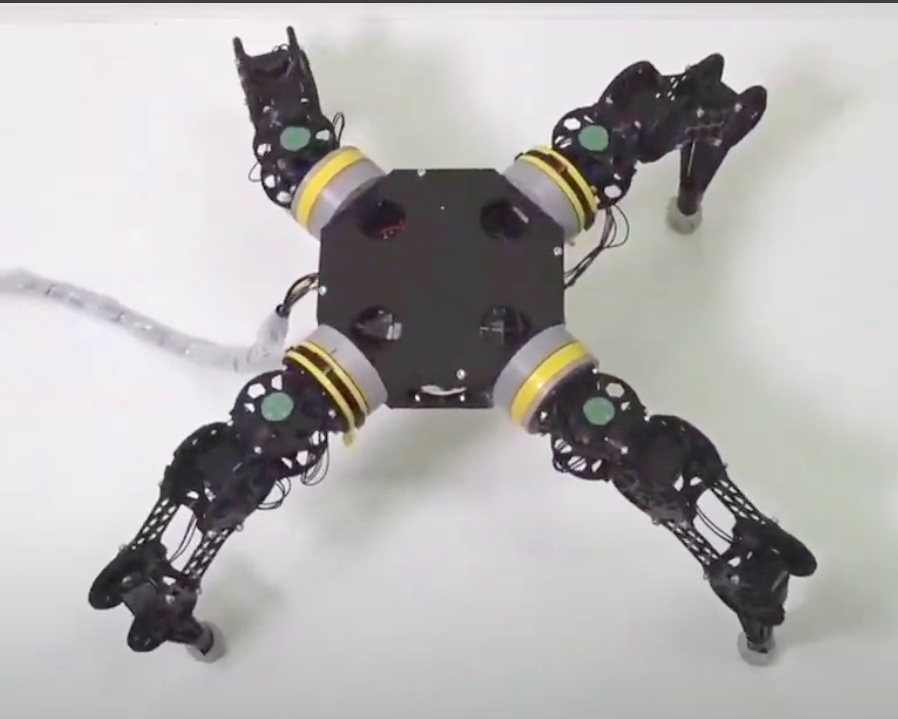
\includegraphics[clip, width=30mm]{./fig/locomotion/45.png}
%   \end{minipage}
%   \begin{minipage}[ht]{0.2\textwidth}
%     \centering
%     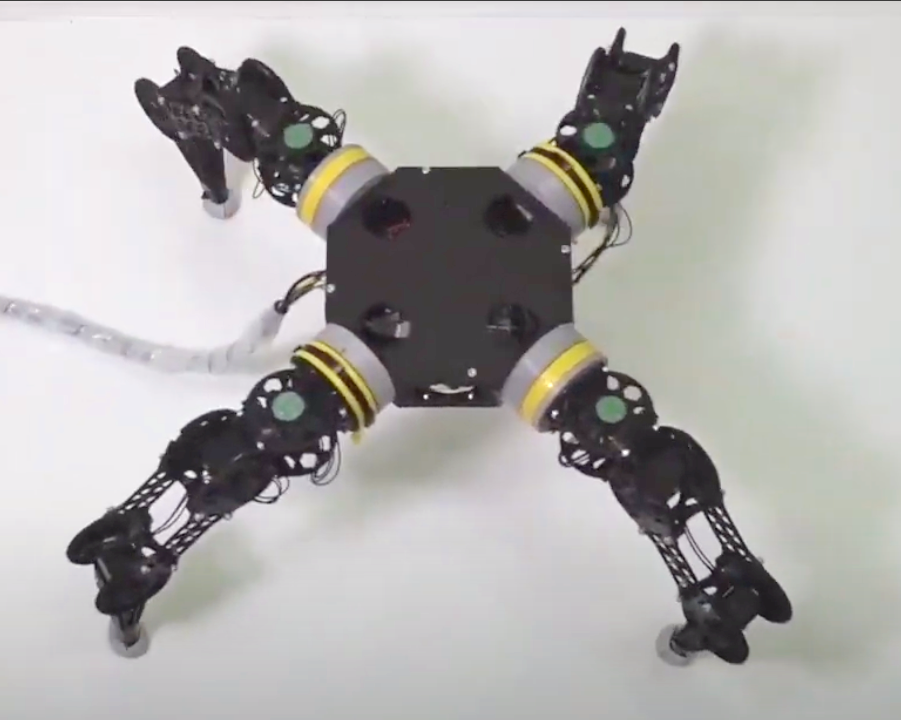
\includegraphics[clip, width=30mm]{./fig/locomotion/46.png}
%   \end{minipage}
%   \begin{minipage}[ht]{0.2\textwidth}
%     \centering
%     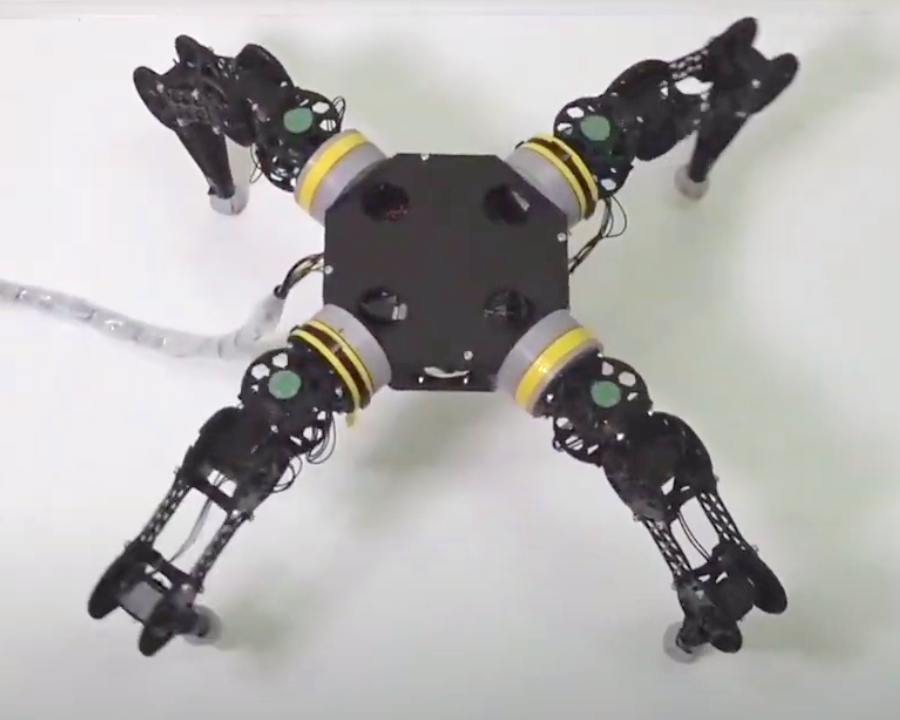
\includegraphics[clip, width=30mm]{./fig/locomotion/47.png}
%   \end{minipage}
% \caption{Walking motion}
% \label{minipage}
% \end{figure}
\end{enumerate}

In addition to the number of module, the type of module also a parameter for motion selection. Moonbot's module contain both leg type and gripper type. By finding the ID dynamixel motor labeled as a gripper type, the robot can recognize the connection of gripper and perform a motion task such as waving and gripping the gripper.\\

\begin{figure}[h]
  \centering
  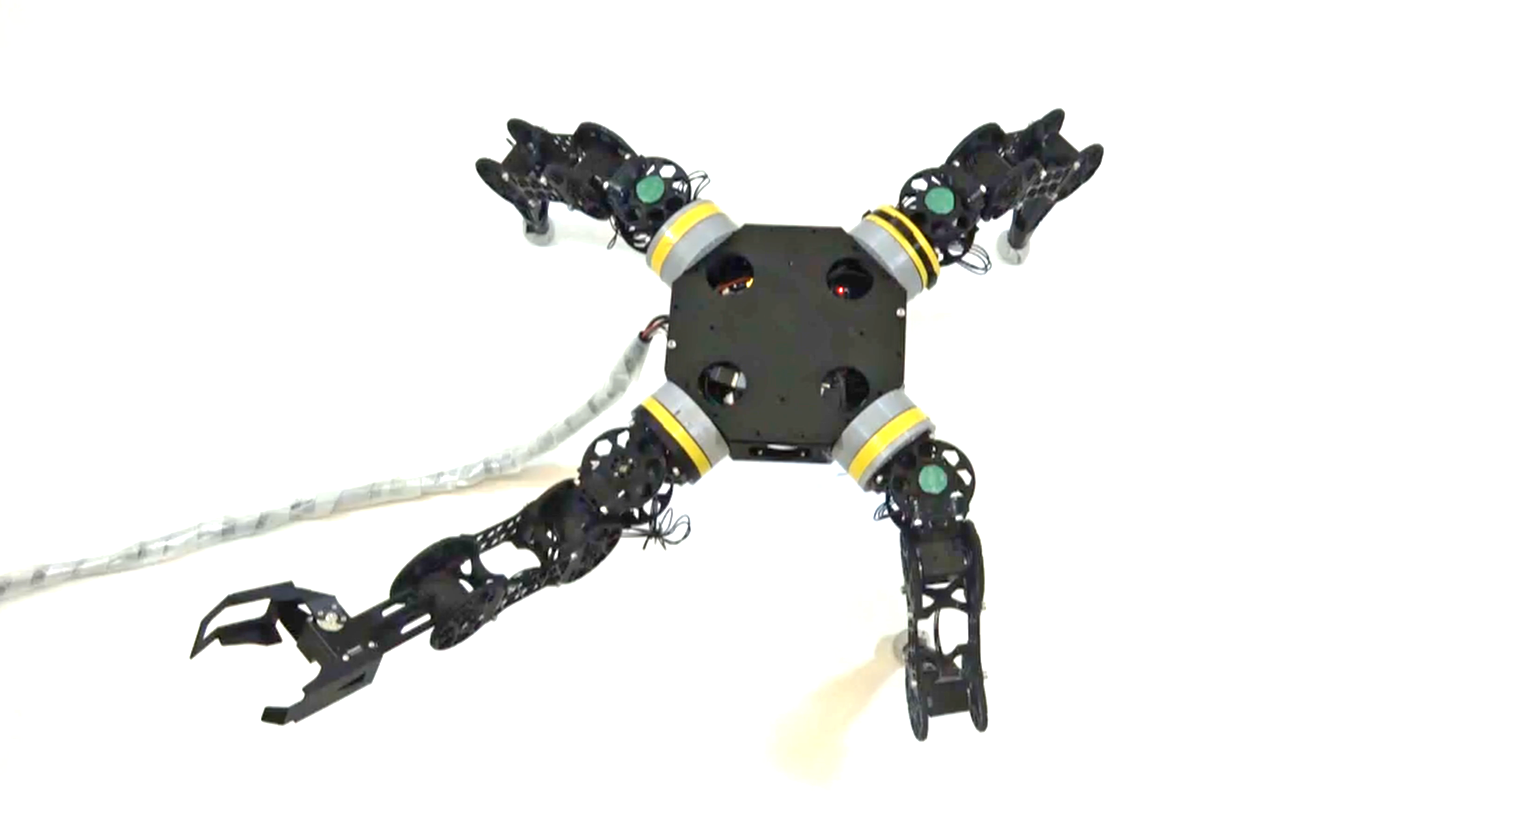
\includegraphics[width=110mm]{./fig/moonbot/grippermoonbot.png}
  \vspace{2mm}
  \caption{Gripper module connect with the Moonbot.}\label{Moonbot gripper}
\end{figure}

\begin{figure}[t]
  \centering
  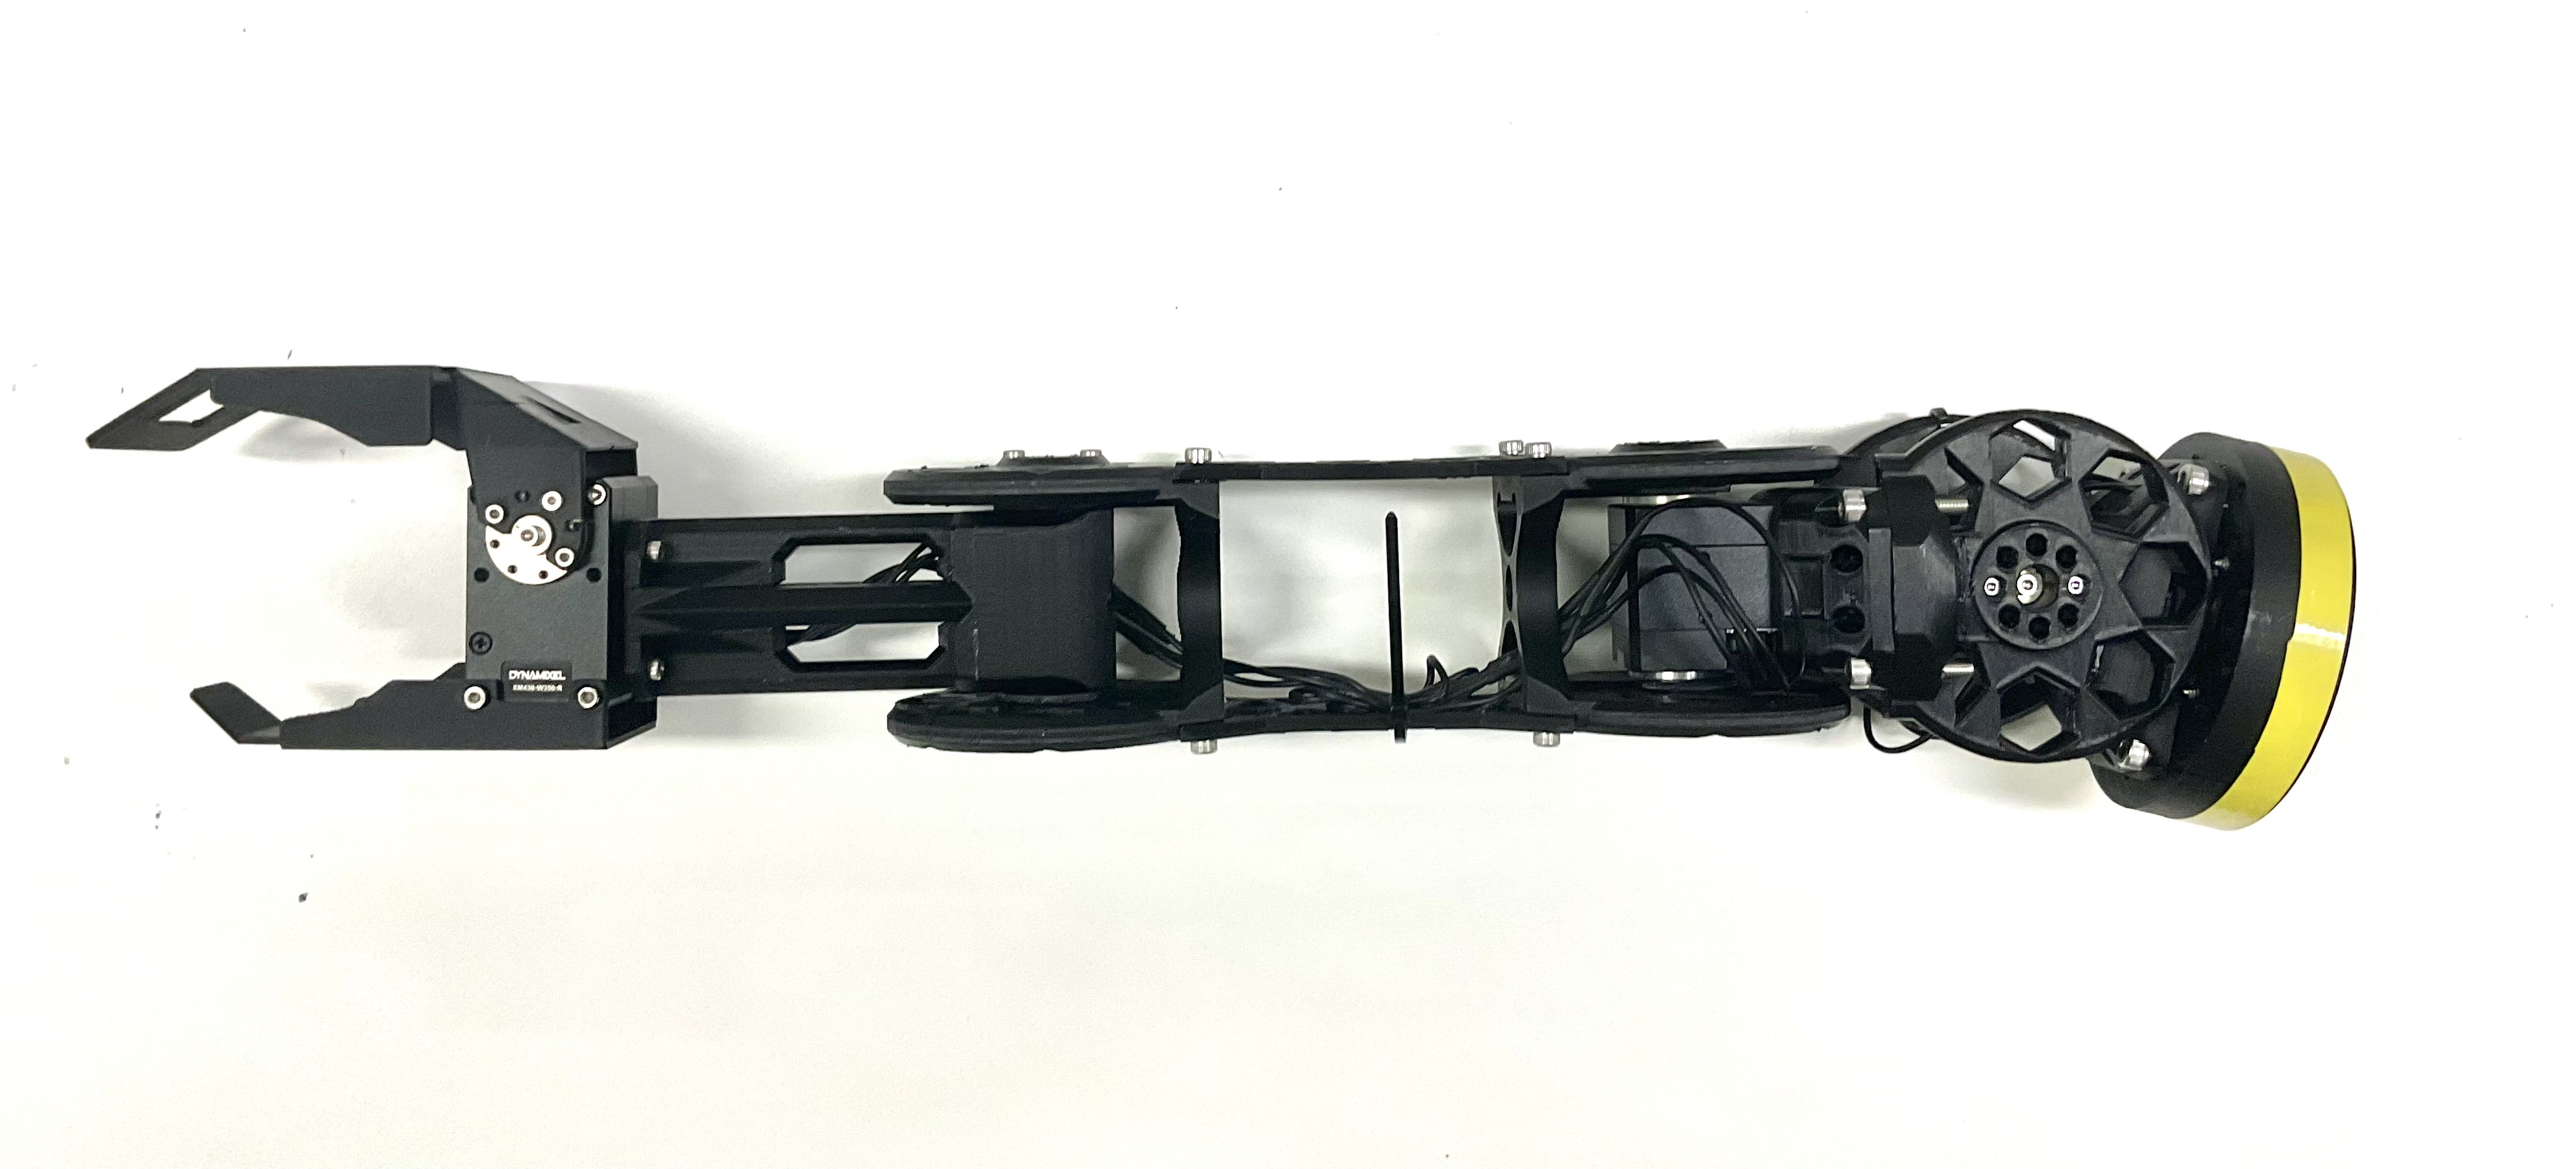
\includegraphics[width=90mm]{./fig/leg_configuration/gripper_module.jpg}
  \vspace{2mm}
  \caption{Motion selection depending on module type.}\label{gripmodule}
\end{figure}

%%% EOF %%%